\section{Boundary conditions}
	\label{sec:bnd_method}
	A simulation must necessarily have finite extent, we need to employ boundary condtions
	to deal with the edges of the simulation. Here we will go through \(3\) different schemes
	corresponding to periodic boundaries, depicted in \cref{fig:bnd}, Dirichlet conditions and Von Neumann conditions.
	Periodic conditions  used when we want to simulate an infinite plasma sheet.
	It is usually used when the plasma sheet is of a much larger extent than the
	length scale of the phenomena we want to investigate, or when the investigated
	dynamics happen away from the edges.
	Dirichlet conditions are useful when the voltage on the edge of the simulation
	can be known beforehand, as it is often in laboratory experiments.
	When the electric field, or alternatively gradient of the voltage, along the edges is known
	von Neumann conditions should be used. The boundary conditions must also be coupled
	with fitting boundary conditions applied to the particles in a full PiC simulation.
	Particle conditions include periodic, bouncing and absorbing boundaries.
	To maintain the design aim of inherent modularity of our PinC model, the boundary conditions
	are defined using ghost points, avoiding different discretization stencils at
	the boundary. This reduces the complexity the smoothers, makes the boundary
	conditions easier to implement and opens the possiblity of using them with other
	solvers.

	%Color scheme
	\tikzstyle{true}=[circle,fill=blue!40,minimum size=25pt,inner sep=0pt]
	\tikzstyle{ghost}=[circle,fill=black!40,minimum size=25pt,inner sep=0pt]
	\tikzstyle{changed} = [circle,fill=red!40,minimum size=25pt,inner sep=0pt]
	\tikzstyle{dirichlet} = [circle,fill=red!40,minimum size=25pt,inner sep=0pt]
	\tikzstyle{periodic} = [circle,fill=green!40,minimum size=25pt,inner sep=0pt]
	\tikzstyle{numbering} = [circle,minimum size=10pt,inner sep=0pt]
	\tikzstyle{edges} = [diamond,fill=black!40,minimum size=25pt,inner sep=0pt]

	\begin{figure}
		\centering
		\begin{subfigure}[b]{0.9\textwidth}
			\centering
			
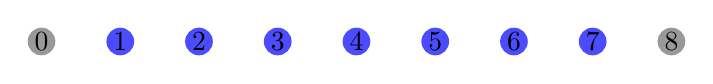
\begin{tikzpicture}%[scale=1, auto,swap]
    %True nodes
    \foreach \pos/\name in 	{{(1,0)/1}, 	{(2,0)/2},	{(3,0)/3},
                             {(4,0)/4},	{(5,0)/5}, {(6,0)/6}, {(7,0)/7}}
    \node[true] (\name) at \pos {$\name$};
    %Ghost nodes
    \node[ghost] (0) at (0,0) {$0$};
    \node[ghost] (8) at (8,0) {$8$};
\end{tikzpicture}

			\caption{A \(1\) dimensional domain with grid points before the boundary conditions has been applied.
			The numbers denote the indexes for the values in the grid array. The blue grid points, (\(1-7\)) represents
			the true grid and the grey points, ($0$ and $8$), is the ghost cell values. The concepts illustrated here can easily be
			expanded to more dimensions.}
			\label{fig:initial}
			% \caption{}
		\end{subfigure}
		\begin{subfigure}[b]{0.9\textwidth}
			\centering
			
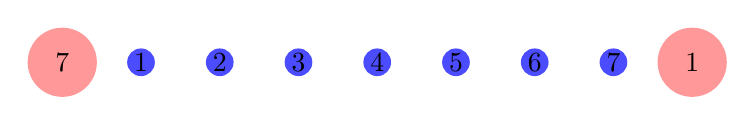
\begin{tikzpicture}%[scale=1, auto,swap]
    %True nodes
    \foreach \pos/\name in 	{{(1,0)/1}, 	{(2,0)/2},	{(3,0)/3},
                             {(4,0)/4},	{(5,0)/5}, {(6,0)/6}, {(7,0)/7}}
    \node[true] (\name) at \pos {$\name$};
    %Ghost nodes
    \node[changed] (0) at (0,0) {$7$};
    \node[changed] (8) at (8,0) {$1$};
\end{tikzpicture}

			\caption{Here periodic boundary conditions has been applied to the \(1\)D domain above. Here and in the following the
			red color means a point has been changed. The ghost points at the edges has been set to equal the
			true grid points at the opposite edge giving periodic boundary conditions.}
			% \caption{}
			\label{fig:periodic}
		\end{subfigure}
		\begin{subfigure}[b]{0.9\textwidth}
			\centering
			
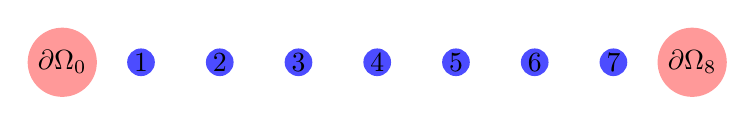
\begin{tikzpicture}%[scale=1, auto,swap]
    %True nodes
    \foreach \pos/\name in 	{{(1,0)/1}, 	{(2,0)/2},	{(3,0)/3},
                             {(4,0)/4},	{(5,0)/5}, {(6,0)/6}, {(7,0)/7}}
    \node[true] (\name) at \pos {$\name$};
    %Ghost nodes
    \node[changed] (0) at (0,0) {$\partial\Omega_0$};
    \node[changed] (8) at (8,0) {$\partial\Omega_8$};
\end{tikzpicture}

			\caption{For Dirichlet boundary conditions we have predetermined values along the edge, this are here represented as the ghost cells
			being set to a given value defined by \(\partial\Omega_i\). The boundary function can be as simple as setting everything along
			the edge to a constant, but it could also be a spatially and time varying function. It is also possible to let it correspond to
			input given by coupled computer model.}
			% \caption{}
			\label{fig:dirichlet}
		\end{subfigure}
		\begin{subfigure}[b]{0.9\textwidth}
			\centering
			
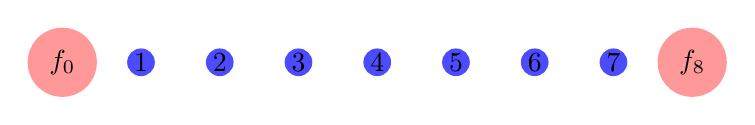
\begin{tikzpicture}%[scale=1, auto,swap]
    %True nodes
    \foreach \pos/\name in 	{{(1,0)/1}, 	{(2,0)/2},	{(3,0)/3},
                             {(4,0)/4},	{(5,0)/5}, {(6,0)/6}, {(7,0)/7}}
    \node[true] (\name) at \pos {$\name$};
    %Ghost nodes
    \node[changed] (0) at (0,0) {$f_0$};
    \node[changed] (8) at (8,0) {$f_8$};
\end{tikzpicture}

			\caption{Von Neumann boundary conditions specifies what the derivative is on the edge. To achieve that we set the ghost points to
			a specified value that will give the wanted derivative when a finite difference method swipes over the point. For the left side
			the function should be set to \(f_0 = u_2 - 2\Delta x A\) and to \(f_8 = u_6 - 2\Delta x A\) for the right side. Here \(A\) is the
			predetermined values that the derivative should correspond to.}
			% \caption{}
			\label{fig:neumann}
		\end{subfigure}
		\caption{An overview of 3 boundary conditions applied to a \(1\)D domain.}
		\label{fig:bnd}
	\end{figure}



\subsection{Periodic Boundaries}
	\label{sec:bnd_periodic}
	With periodic boundary conditions we want the boundary on one side to be equal
	to the field on the other side of the plasma. For the \(1\)D case, see \cref{fig:periodic},
	this can be written as

	\begin{equation}
		\nabla^2 \phi = -\rho \qquad \Omega = [0,L]
	\end{equation}

	With boundaries

	\begin{equation}
		\phi(0) = \phi(L)
	\end{equation}

	Here we should note that this is very similar to what happens between the subdomains
	in a Domain Partitioning parallelization scheme, so often the same algorithm and code
	can be reused to achieve periodic boundary conditions.

	Solutions for the contineous problem with periodic boundary conditions exists only if
	the \textit{compatibility condition} \citep{trottenberg_multigrid_2000}

	\begin{equation}
			\int_\Omega \rho\differential \vb{x} = 0
	\end{equation}

	is held. This means that the total charge in the domain must be zero, which
	is often true in plasma due to quasi-neutrality.

	To ensure a unique discretized solution need to set the integration constant, this can be done
	by setting a \textit{global constraint} on the solution

	\begin{equation}
		\sum_{\Omega} \phi = 0 \label{eq:global_constraint}
	\end{equation}

\subsection{Dirichlet Boundaries}
	With Dirichlet conditions the boundaries of the potential are known and given by a function,
	\(\partial \phi = f\). Then a \(1\)D problem, \cref{fig:dirichlet} , is represented by

	\begin{equation}
		\nabla^2 \phi = -\rho \qquad \Omega = [0,L]
	\end{equation}
	with boundaries
	\begin{equation}
		\phi(0) =  f(0), \qquad f(L) =   f(L)
	\end{equation}


\subsection{Neumann Boundaries}
	Now we assume we know the gradient of the potential along the boundary, \(\nabla\phi_{\partial \Omega} = f\).
	This is often used in hydrodynamics to represent reflecting boundaries.
	Then our \(1\)D example problem will look like

	\begin{equation}
		\nabla^2 \phi = -\rho \qquad \Omega = [0,L] \label{eq:1D_poisson}
	\end{equation}
	with boundaries
	\begin{equation}
		\partial \phi(0) = f(0), \qquad \partial \phi(L) = f(L)
	\end{equation}

	The boundary condition is then stated as a gradient and we need to approximate it
	to \(\phi\) to use it in the poisson equation, \cref{eq:1D_poisson}.
	We do this by a \(2\)nd order central difference to the gradient.

	\begin{equation}
		\pdv{\phi(x)}{x} = \frac{\phi(x +\Delta x ) - \phi(x -\Delta x )}{2\Delta x} = f(x)
	\end{equation}

	At the lower boundary, \(x=0\), this can then be written as
	\begin{equation}
		\phi(-\Delta x) = \phi(\Delta x) - 2\Delta x f(0) \label{eq:neumann_lower}
	\end{equation}
	and at the upper
	\begin{equation}
		\phi(L + \Delta x) = \phi(L + \Delta x) - 2\Delta x f(L) \label{eq:neumann_upper}
	\end{equation}

	With our discretization, where the internal cell sizes are \(1\), the \(\phi(-\Delta x)\)
	correspond directly to a ghost cell. So we can implement the Neumann boundary conditions
	easily by setting the ghost cells equal to \cref{eq:neumann_lower,eq:neumann_upper},
	see \cref{fig:neumann}.
	This scheme completely avoids any modification of the smoother stencils at the boundaries.

	\subsection{Boundaries in Multigrid}
	The multigrid algorithm solves the problem on several discretization levels.
	Due to this we need to represent the boundaries on the coarser grid levels as well.

	\subsubsection{Periodic}
		Since the periodic boundary conditions can be tougth of to set the domain next
		a copy of itself the boundary treatment will remain equal on the coarser
		grids. It should also be mentioned that the \textit{global constraint}, \cref{eq:global_constraint},
		only needs to be set on the coarsest grids to achieve good convergence
		rates \citep{trottenberg_multigrid_2000}.

	\subsubsection{Dirichlet}
		The Dirichlet condition specifies the potential at the boundaries. Since the conditions
		should apply to the problem at all coarseness levels, we need a restriction
		operator specific to the boundary.

		The easiest boundary restriction operator is direct injection, letting each
		coarse grid point correspond to a grid point on the boundary of the finer grid.
		This is often sufficient, especially in the case of spatially constant boundaries.
		If the boundaries are constant in time, the computing time can be saved by computing the boundaries for all levels
		once at the start of the simulation.

		If the boundaries are more complicated first or second order interpolation
		could be used to restrict them.

	\subsubsection{Neumann}
		The Neumann conditions are dependent on the next to outermost grid point,
		i.e. grid point \(2\) in \cref{fig:neumann} on the lower side,
		because of this they will have to be recomputed each time they are used.
		But still the function \(f\) should be restricted seperately from the
		finer grid restriction.


	\subsection{Mixed Conditions}
		All the boundary conditions can be implemented with the use of ghost cells,
		this enables the use of the \(5\)-point stencil for the smoothers. This
		greatly simplifies mixed boundary conditions, the boundaries are set on the
		ghost layer of the grid seperately, then the smoother runs. Here it should
		be noted that the boundaries need to be reset for each halfcycle in GS-RB.

		As can be seen in \cref{fig:mixed} we do not have to care for the corners
		of the domain, as long as we are using a \(5\)-point stencil. This allows us to not
		need to care of which boundary conditions takes precedence when they clash.
		For a higher order, or different, stencils the corner ghost cells may be important
		and the mixing of boundary conditions need to be given extra care.

		\begin{figure}
			\centering
			
%Figure
\tikzstyle{true}=[circle,fill=blue!70,minimum size=10pt,inner sep=0pt]
\tikzstyle{ghost}=[circle,fill=black!40,minimum size=10pt,inner sep=0pt]
\tikzstyle{numbering} = [circle,minimum size=10pt,inner sep=0pt]


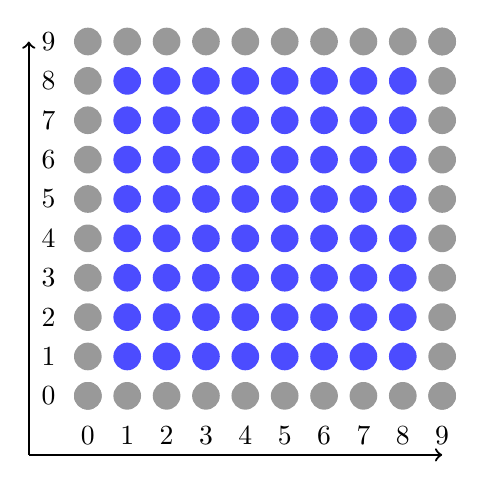
\begin{tikzpicture}[scale=0.50, auto,swap]
    %Adding the ghost nodes along the edges
    \foreach \pos/\name in 	{{(0,0)/},	{(1,0)/}, 	{(2,0)/},	{(3,0)/},
                             {(4,0)/},	{(5,0)/}, 	{(6,0)/},	{(7,0)/},
                             {(8,0)/},	{(9,0)/}}
    \node[ghost] (\name) at \pos {$\name$};
    \foreach \pos/\name in 	{			{(0,1)/}, 	{(0,2)/},		{(0,3)/},
                            {(0,4)/},	{(0,5)/}, 	{(0,6)/},		{(0,7)/},
                            {(0,8)/}, 	{(0,9)/}}
    \node[ghost] (\name) at \pos {$\name$};
    \foreach \pos/\name in 	{{(0,0)/},	{(1,9)/}, 	{(2,9)/},		{(3,9)/},
                             {(4,9)/},	{(5,9)/}, 	{(6,9)/},		{(7,9)/},
                             {(8,9)/}, 	{(9,9)/}}
    \node[ghost] (\name) at \pos {$\name$};
    \foreach \pos/\name in 	{{(9,0)/},	{(9,1)/}, {(9,2)/},		{(9,3)/},
                             {(9,4)/},	{(9,5)/}, {(9,6)/},		{(9,7)/},
                             {(9,8)/},	{(9,9)/}}
    \node[ghost] (\name) at \pos {$\name$};
    %Adding true grid
    \foreach \pos/\name in 	{{(1,1)/},	{(2,1)/},	{(3,1)/},	 {(4,1)/},
                            {(5,1)/}, 	{(6,1)/},	{(7,1)/},	 {(8,1)/}}
    \node[true] (\name) at \pos {$\name$};
    \foreach \pos/\name in 	{{(1,2)/},	{(2,2)/},	{(3,2)/},	 {(4,2)/},
                            {(5,2)/}, 	{(6,2)/},	{(7,2)/},	 {(8,2)/}}
    \node[true] (\name) at \pos {$\name$};
    \foreach \pos/\name in 	{{(1,3)/},	{(2,3)/},	{(3,3)/},	 {(4,3)/},
                            {(5,3)/}, 	{(6,3)/},	{(7,3)/},	 {(8,3)/}}
    \node[true] (\name) at \pos {$\name$};
    \foreach \pos/\name in 	{{(1,4)/},	{(2,4)/},	{(3,4)/},	 {(4,4)/},
                            {(5,4)/}, 	{(6,4)/},	{(7,4)/},	 {(8,4)/}}
    \node[true] (\name) at \pos {$\name$};
    \foreach \pos/\name in 	{{(1,5)/},	{(2,5)/},	{(3,5)/},	 {(4,5)/},
                            {(5,5)/}, 	{(6,5)/},	{(7,5)/},	 {(8,5)/}}
    \node[true] (\name) at \pos {$\name$};
    \foreach \pos/\name in 	{{(1,6)/},	{(2,6)/},	{(3,6)/},	 {(4,6)/},
                            {(5,6)/}, 	{(6,6)/},	{(7,6)/},	 {(8,6)/}}
    \node[true] (\name) at \pos {$\name$};
    \foreach \pos/\name in 	{{(1,7)/},	{(2,7)/},	{(3,7)/},	 {(4,7)/},
                            {(5,7)/}, 	{(6,7)/},	{(7,7)/},	 {(8,7)/}}
    \node[true] (\name) at \pos {$\name$};

    \foreach \pos/\name in 	{{(1,8)/},	{(2,8)/},	{(3,8)/},	 {(4,8)/},
                            {(5,8)/}, 	{(6,8)/},	{(7,8)/},	 {(8,8)/}}
    \node[true] (\name) at \pos {$\name$};
    %Adding numbering
    \foreach \pos/\name in 	{{(0,-1)/0},	{(1,-1)/1}, 	{(2,-1)/2},	{(3,-1)/3},
                             {(4,-1)/4},	{(5,-1)/5}, 	{(6,-1)/6},	{(7,-1)/7},
                             {(8,-1)/8},	{(9,-1)/9}}
    \node[numbering] (\name) at \pos {$\name$};
    \foreach \pos/\name in 	{{(-1,0)/0},	{(-1,1)/1}, 	{(-1,2)/2},		{(-1,3)/3},
                            {(-1,4)/4},		{(-1,5)/5}, 	{(-1,6)/6},		{(-1,7)/7},
                            {(-1,8)/8}, 	{(-1,9)/9}}
    \node[numbering] (\name) at \pos {$\name$};
    \draw[->, black, thick] (-1.5,-1.5) -- (9,-1.5);
    \draw[->, black, thick] (-1.5,-1.5) -- (-1.5,9);
\end{tikzpicture}

			\caption{This is a \(2\)D domain with mixed boundary conditions, along the $x$-axis there are
			periodic boundary conditions, green ghost points, and the $y$-axis there are dirichlet boundary conditions, red ghost points. If
			the smoothers are using a 5 point discretization stencil the corners, grey diamonds, are neglected when
			computing the inner, i.e. true,  grid.}
			\label{fig:mixed}
		\end{figure}
